\item[9] As soon as the grades for CPSC 121 have been submitted to the department, Geoff will celebrate the start of his summer break by using his car to draw perfect circles of melted rubber in the parking lot across the street from ICCS. He draws his doughnuts according to the following rules:
\begin{itemize}
\item No circle can touch or intersect the (rectangular) boundaries of the parking lot, and
\item Each new circle must intersect with the other circles such that it produces the maximum number of separate regions in the parking lot.
\end{itemize}

The maximum number of regions produced by $n$ circles (including the outside of the circles) for some small values of $n$ are shown below:

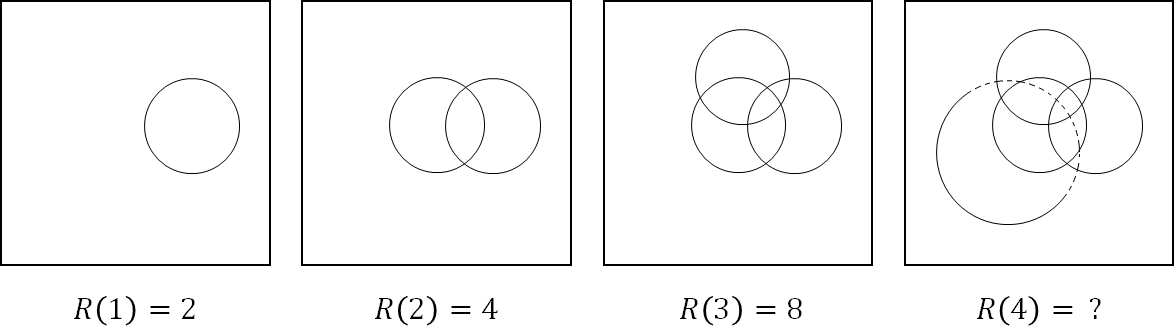
\includegraphics[width=15.0cm]{images/circlepartitions.png}

  \begin{question}{a.}[3]
  \item[1] What is the value of $R(4)$? You should trace the dotted portion of the circle to see exactly how regions are created. If your answer does not seem to fit the obvious pattern, you are probably on the right track.
  \\{\color{NavyBlue}
  \\R(4) = 14
  \\}
  
  \item[2] \label{doughnut-rec} The arrangement of circles that achieves the maximum number of regions has the property that every pair of circles intersects twice.
Given this fact, complete the following recurrence relation for $R(n)$:
{\color{NavyBlue}
\begin{align*}
R(1) &= 2\\
R(n) &= R(n-1) + 2(n-1) \qquad \text{for $n>1$}
\end{align*}
  }
  \item[6] Geoff has determined (by techniques he learned in CPSC 221) that the formula for the maximum number of circles is $R(n)=n^{2} - n + 2$.
  
  Using mathematical induction and your recursive definition found in part (\ref{doughnut-rec}), prove that this formula is correct for all $n \geq 1$.
  \begin{Questions}
  \\{\color{NavyBlue}
  \\Proof:
 \\
 \\Part 1: Base case
 \\Using formula: $R(2) = 2^2-2+2=4$
 \\Using recursive definition: $R(2) = R(1)+2*(2-1) = 2+2= 4$ 
 \\
 \\Part 2:
 \\Assuming $R(n)=n^{2} - n + 2$ and $R(n) = R(n-1) + 2(n-1)$ are true:
 \begin{gather}
 R(n+1)=(n+1)^{2} - (n+1) + 2\\
 R(n+1)=R(n)+2(n+1-1)=n^{2} - n + 2+2(n)\\
 (n+1)^{2} - (n+1) + 2=n^{2} - n + 2+2(n)\\
 (n+1)^{2} - (n+1) + 2=n^{2} +n+2\\
 n^{2}+2n+1 - (n+1) + 2=n^{2} +n+2\\
 n^{2} +n+2=n^{2} +n+2
 \end{gather} 
 \\
 \\Line 14-15 states out the two forms of R(n+1) equations. Line 16 equates the two forms. Line 17 combines like terms of RHS. Line 18-19 expands exponents and combine like terms of LHS.
 \\
 \\We have proved that the base case is true and n+1 case is true when n case is true, therefore the induction proof is complete.
 \\ }
 \begin{figure}[H]
\begin{verbatim}  

________/\\\_______        __/\\\\\\\\\\\\\\\_        __/\\\\\\\\\\\\____        
 _____/\\\\/\\\\____        _\/\\\///////////__        _\/\\\////////\\\__       
  ___/\\\//\////\\\__        _\/\\\_____________        _\/\\\______\//\\\_      
   __/\\\______\//\\\_        _\/\\\\\\\\\\\_____        _\/\\\_______\/\\\_     
    _\//\\\______/\\\__        _\/\\\///////______        _\/\\\_______\/\\\_    
     __\///\\\\/\\\\/___        _\/\\\_____________        _\/\\\_______\/\\\_   
      ____\////\\\//_____        _\/\\\_____________        _\/\\\_______/\\\__  
       _______\///\\\\\\__        _\/\\\\\\\\\\\\\\\_        _\/\\\\\\\\\\\\/___ 
        _________\//////___        _\///////////////__        _\////////////_____
\end{verbatim}
\caption{Another blessed QED to end another blessed proof}
\end{figure}
  \vfill
  \vfill\eject
  \clearpage
  
  \end{Questions}
  \end{question}
